\chapter{Introduction}
\label{cpt:introduction}

Rendering is one of the three fundamental problems in computer graphics accompany by modeling and simulation. It builds the bridge between the 3D virtual world and the images showed on display. In recent decades, path-tracing-based photorealistic rendering became a general and standard technique in the movie and animation industries. Most commercial Ads using rendered images instead of captured photos. We know how light interacts with surfaces and participating media from the principles of physical rules (especially in optics). As a result, an indistinguishable virtual world could be established using computers.  

As we enjoy the realism of the virtual world from pioneers' works, more challenges await us. The real world contains many types of materials, while only a few can be modeled in renderings, such as diffuse, specular, transparent, and so on. In most cases, people can quickly tell the object in an image is rendered since it looks \emph{too perfect to be true}. The over-perfect issue is because of details missing for complex materials (See Figure \ref{fig:introduction:material}). Artists always hack the macro appearance with texture mapping or mix the existing appearance models, which is ad-hoc and unrealistic since microstructures of a surface or medium bring undesirable light interaction and further affect the macro appearance. In this dissertation, we first address a more general but efficient way to handle complex surface reflectance (layered material) and volumetric scattering with micro details.

\begin{figure}[h]
	\centering
	\setlength{\resLen}{3.in}
	\addtolength{\tabcolsep}{0pt}
	\begin{tabular}{cc}
		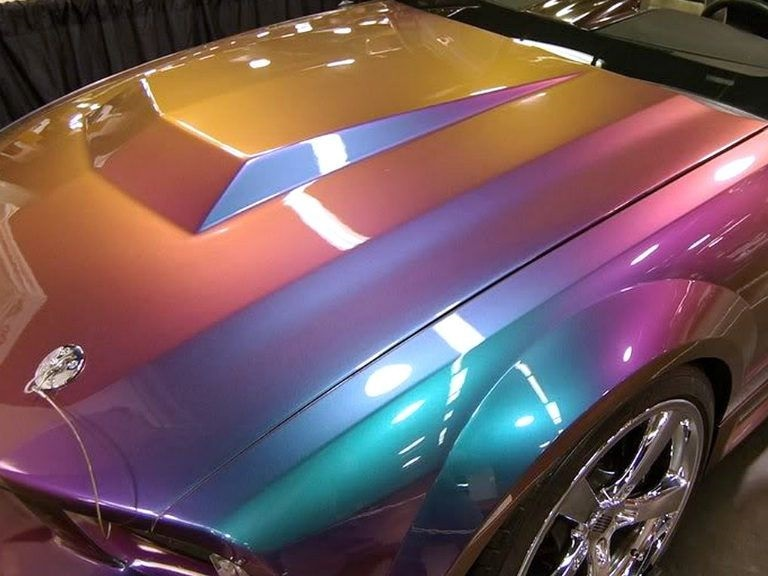
\includegraphics[width=\resLen]{other/car.jpg} & 
		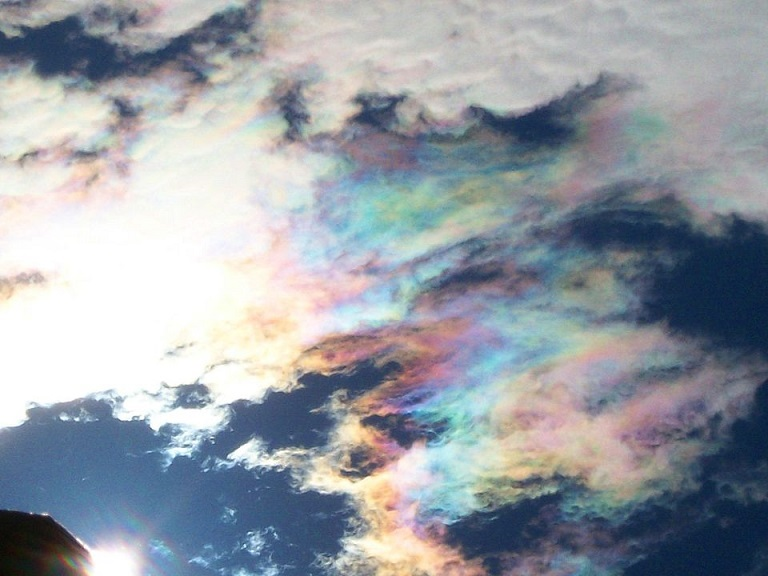
\includegraphics[width=\resLen]{other/cloud.jpg} 
	\end{tabular}
	\caption[Examples of complex materials]{\label{fig:introduction:material}
		\textbf{Examples of complex materials} in real life.
		\textbf{Left:} car with `mermaid' paint; \textbf{Right:} cloud iridescence phenomena.
	}
\end{figure}

To better represent the real world, another challenge is to acquire the geometry of the objects, the physical properties of the materials, and the scene illumination from observed measurements more accurately and efficiently. This inverse process of rendering (inverse rendering) becomes a popular topic in Computer Graphics and Computer Vision. In industry, artists use \emph{photoshop} to create material maps or use some heavy capturing systems to acquiring them. In the second half of this dissertation, we will focus on material properties estimation by just giving a small number of input cellphone captures.

To summarize, we develop a smart technique to render layered materials, a framework to compute scatterings in participating media based on wave optics, an optimization-based method for SVBRDF (Spatially Varying Bidirectional Reflectance Distribution Functions,
as will be introduced in Chapter \ref{cpt:background}) reconstruction and then extend it to posterior estimation using Bayesian inference.
These techniques were presented at multiple ACM SIGGRAPH (Asia) conferences \cite{guo2018position, guo2021beyond, guo2020materialgan} and Pacific Graphics \cite{guo2020bayesian}. Our specific contributions include:

\paragraph{Position-free Monte Carlo simulation for arbitrary layered BSDFs.}
Real-world materials are often layered: metallic paints, biological tissues, and many more. Variation in the interface and volumetric scattering properties of the layers leads to a rich diversity of material appearances from anisotropic highlights to complex textures and relief patterns. However, simulating light-layer interactions is a challenging problem. Past analytical or numerical solutions either introduce several approximations and limitations, or rely on expensive operations on discretized BSDFs, preventing the ability to freely vary the layer properties spatially. 
In Chapter \ref{cpt:layeredbsdf}, we introduce a new unbiased layered BSDF model based on Monte Carlo simulation, whose only assumption is the layer assumption itself. Our novel position-free path formulation is fundamentally more powerful at constructing light transport paths than generic light transport algorithms applied to the special case of flat layers, since it is based on a product of solid angle instead of area measures, so does not contain the high-variance geometry terms needed in the standard formulation. We introduce two techniques for sampling the position-free path integral, a forward path tracer with next-event estimation and a full bidirectional estimator. We show a number of examples, featuring multiple layers with surface and volumetric scattering, surface and phase function anisotropy, and spatial variation in all parameters.

\paragraph{Beyond Mie theory: systematic computation of bulk scattering parameters based on microphysical wave optics.}
Light scattering in participating media and translucent materials is typically modeled using the radiative transfer theory. Under the assumption of independent scattering between particles, it utilizes several bulk scattering parameters to statistically characterize light-matter interactions at the macroscale. To calculate these parameters based on microscale material properties, the Lorenz-Mie theory has been considered the gold standard.
In Chapter \ref{cpt:waveoptics}, we present a generalized framework capable of systematically and rigorously computing bulk scattering parameters beyond the far-field assumption of Lorenz-Mie theory. Our technique accounts for microscale wave-optics effects such as diffraction and interference as well as interactions between nearby particles. Our framework is general, can be plugged in any renderer supporting Lorenz-Mie scattering, and allows arbitrary packing rates and particles correlation; we demonstrate this generality by computing bulk scattering parameters for a wide range of materials, including anisotropic and correlated media.

\paragraph{MaterialGAN: reflectance capture using a generative SVBRDF model.}
We address the problem of reconstructing spatially-varying BRDFs from a small set of image measurements. This is a fundamentally under-constrained problem, and previous work has relied on using various regularization priors or on capturing many images to produce plausible results.
In Chapter \ref{cpt:svbrdf}, we present \emph{MaterialGAN}, a deep generative convolutional network based on StyleGAN2, trained to synthesize realistic SVBRDF parameter maps. We show that MaterialGAN can be used as a powerful material prior in an inverse rendering framework: we optimize in its latent representation to generate material maps that match the appearance of the captured images when rendered. We demonstrate this framework on the task of reconstructing SVBRDFs from images captured under flash illumination using a hand-held mobile phone. Our method succeeds in producing plausible material maps that accurately reproduce the target images, and outperforms previous state-of-the-art material capture methods in evaluations on both synthetic and real data. Furthermore, our GAN-based latent space allows for high-level semantic material editing operations such as generating material variations and material morphing.

\paragraph{A Bayesian Inference Framework for Procedural Material Parameter Estimation.}
Procedural material models have been gaining traction in many applications thanks to their flexibility, compactness, and easy editability.
In Chapter \ref{cpt:bayesian}, we explore the inverse rendering problem of procedural material parameter estimation from photographs, presenting a unified view of the problem in a Bayesian framework. In addition to computing point estimates of the parameters by optimization, our framework uses a Markov Chain Monte Carlo approach to sample the space of plausible material parameters, providing a collection of plausible matches that a user can choose from, and efficiently handling both discrete and continuous model parameters. To demonstrate the effectiveness of our framework, we fit procedural models of a range of materials---wall plaster, leather, wood, anisotropic brushed metals and layered metallic paints---to both synthetic and real target images.

The dissertation is organized as follows. We first introduce the basic background on light transport, wave-optics and BRDF representations in Chapter \ref{cpt:background}. From Chapters \ref{cpt:layeredbsdf} to \ref{cpt:bayesian}, we present technical details of our layered rendering, wave-optics bulk scattering, SVBRDF reconstruction and procedure model estimation, respectively. Finally, we present our conclusion and discuss future research directions in Chapter \ref{cpt:conclusion}.